\documentclass{article}
\usepackage{../../fasy-hw}

\title{Computational Geometry, Homework \hwnum}
\collab{n/a}

%% Instructor: update these macros:
\renewcommand{\hwnum}{4}
\date{due: Tuesday, 11 April 2023}

%% Student: update this macro:
\author{\todo{Your Name Here}}

\begin{document}

\maketitle

This homework assignment should be
submitted as a single PDF file to D2L.

General homework expectations:
\begin{itemize}
    \item Homework should be typeset using LaTex.
    \item Answers should be in complete sentences and proofread so that they
        make sense without seeing the question.
    \item You will not plagiarize, nor will you share your written solutions
        with classmates. (But, discussing the questions is highly encouraged).
    \item List collaborators at the start of each question using the
        \texttt{collab} command.
    \item Put your answers where the \texttt{todo} command currently is (and
        remove the \texttt{todo} macro, but not the word \texttt{Answer}).
    \item If you are asked to come up with an algorithm, you are
        expected to give an efficient algorithm (brute-force solutions will not
        be accepted). With your algorithm, please provide the following:
        \begin{itemize}
            \item \emph{What}: A prose explanation of the problem and the algorithm,
                including a description of the input/output.  Be sure to state
                your GP assumptions.
            \item \emph{How}: Describe how the algorithm works clearly.
                Including pseudocode may helpful.
            \item \emph{How Fast}: Runtime, along with the derivation.  (Or, at
                the very least, a proof of termination using a decrementing
                function).  You only need to specify the space complexity if the
                problem asks for it.
           \item \emph{Why}: Brief justification of why the algorithm works.
               Often, this will include a statement of the loop invariant for each
               (outer-most) loop, or recursion invariant for each recursive function.
        \end{itemize}
\end{itemize}

{\bf David Mount's tips for writing up homework solutions}:
Remember that your description is intended to be read by a
human, not a compiler, so conciseness and clarity are preferred over technical
details.  Unless otherwise stated, you may use any results from class, or
results from any standard textbook on algorithms and data structures. Also, you
may use results from geometry that: (1) have been mentioned in class, (2) would
be known to someone who knows basic geometry or linear algebra, or (3) is
intuitively obvious. If you are unsure, please feel free to check with me.

Giving careful and rigorous proofs can be quite cumbersome in geometry, and so
you are encouraged to use intuition and give illustrations whenever appropriate.
Beware, however, that a poorly drawn figure can make certain erroneous
hypotheses appear to be ``obviously correct.''

Throughout the semester, unless otherwise stated, you may assume that input
objects are in general position. For example, you may assume that no two points
have the same x-coordinate, no three points are collinear, no four points are
co-circular. Also, unless otherwise stated, you may assume that any geometric
primitive involving a constant number of objects each of constant complexity can
be computed in $\Theta(1)$ time


{\bf Acknowledgement}: the homework problems were adapted from assignments of David
Millman, which, in turn, were adaptations of problems by David Mount and Carola
Wenk.

%%%%%%%%%%%%%%%%%%%%%%%%%%%%%%%%%%%%%%%%%%%%%%%%%%%%%%%%%%%%%%%%%%%%%%%%%%%%%%
\collab{\todo{}}
\nextprob{Randomized Analysis}

Consider the following algorithm:

\begin{verbatim}
    FindMax(A,n){
        // Finds maximum in set A of n numbers
        if(n==1) return the single number in A
        else {
            x = extract random element from A // in constant time; x is removed from
            A
            y = FindMax(A,n-1)
            if(x<=y) return y;
            else
            Compare x with all remaining elements in A and return the maximum
        }
    }
\end{verbatim}

\begin{enumerate}

    \item Argue that this algorithm is correct, and give its worst-case
        runtime. (The runtime is proportional to the number of comparisons made.)

        \todo{replace this TODO with your answer}

    \item Compute the expected runtime of this algorithm.  (Hint:
        Introduce an indicator random variable for executing the else branch in the
        $i$-th step, and use backwards analysis to simplify the analysis.)

        \todo{replace this TODO with your answer}

\end{enumerate}


\todo{replace this TODO with your answer}
%%%%%%%%%%%%%%%%%%%%%%%%%%%%%%%%%%%%%%%%%%%%%%%%%%%%%%%%%%%%%%%%%%%%%%%%%%%%%%

%%%%%%%%%%%%%%%%%%%%%%%%%%%%%%%%%%%%%%%%%%%%%%%%%%%%%%%%%%%%%%%%%%%%%%%%%%%%%%
\collab{\todo{}}
\nextprob{Linear Programming}

Explain how to solve each of the following problems in linear (expected) time.
Each can be modeled as a linear programming (LP) problem, perhaps with some
additional pre- and/or post- processing. In each case, explain how the problem
is converted into an LP instance and how the answer to the LP instance is
used/interpreted to solve the stated problem.

\begin{enumerate}

    \item You are given two point sets $P = \{p_1,\ldots,p_n\}$ and $Q =
        \{q_1,\ldots,q_m\}$ in the plane, and you are told that they are
        separated by a vertical line $x = x_0$, with $P$ to the left and $Q$ to
        the right (see Fig. a). Compute the line equations of the two
        ``crossing tangents,'' that is, the lines $\ell_1$ and $\ell_2$ that are
        both supporting lines for $\rm{conv}(P)$ and $\rm{conv}(Q)$ such that
        $P$ lies below $\ell_1$ and above $\ell_2$ and the reverse holds for
        $Q$. (Note that you are not given the hulls, just the point sets.) Your
        algorithm should run in time $O(n + m)$.

        \begin{figure}[h]
            \centering
            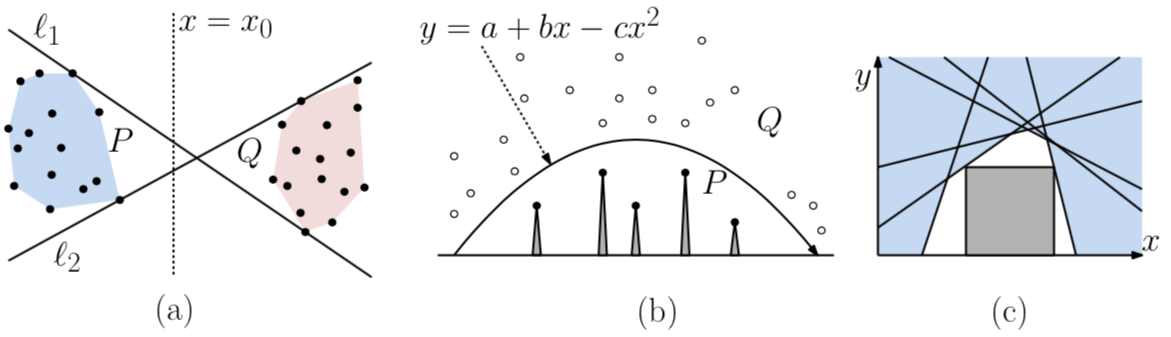
\includegraphics[width=0.75\textwidth]{lp}
            \caption{Problem 3: LP applications}
        \end{figure}

        \paragraph{Answer}
        \todo{replace this TODO with your answer}

    \item You have a cannon in $\R^2$. It has three controls labeled ``a'' ``b,''
        and ``c''. A projectile shot from this cannon travels along the
        parabolic arc $y = a + bx - cx^2$. You are asked to determine whether it
        is possible to adjust the controls so that the projectile travels above
        a set of $n$ building tops, represented by a point set $P = \{p_1,
        \ldots , p_n\}$ and beneath a set of $m$ floating balloons, represented
        by a point set $Q = \{q_1, \ldots , q_m\}$ (see Fig. b)). Your algorithm
        should run in time $O(n + m)$. (I do not care where the cannon is
        actually located. If your solution is based on some assumption about the
        cannon's location, please state this.)

        \paragraph{Answer}
        \todo{replace this TODO with your answer}

    \item You are given a set of $n$ halfplanes $H = \{h_1,\ldots,h_n\}$, where
        $h_i$ is given as a pair $(a_i,b_i)$ and it consists of all the points
        of the plane that lie on or beneath the line $y = a_ix + b_i$. Compute
        the axis-parallel square of the largest side length whose lower edge
        lies on the x-axis (see Fig.~c). If no such square exists, your
        algorithm should indicate this.


        \paragraph{Answer}
        \todo{replace this TODO with your answer}

\end{enumerate}

%%%%%%%%%%%%%%%%%%%%%%%%%%%%%%%%%%%%%%%%%%%%%%%%%%%%%%%%%%%%%%%%%%%%%%%%%%%%%%

%%%%%%%%%%%%%%%%%%%%%%%%%%%%%%%%%%%%%%%%%%%%%%%%%%%%%%%%%%%%%%%%%%%%%%%%%%%%%%
\collab{\todo{}}
\nextprob{Find Voronoi Sites}

Suppose we are given a subdivision of the plane into $n$ convex regions. We
suspect that this subdivision is a Voronoi diagram, but we do not know the
sites. Develop an algorithm that finds a set of $n$ point sites whose Voronoi
diagram is exactly the given subdivision, if such a set exists.

\paragraph{Answer}

\todo{replace this TODO with your answer}
%%%%%%%%%%%%%%%%%%%%%%%%%%%%%%%%%%%%%%%%%%%%%%%%%%%%%%%%%%%%%%%%%%%%%%%%%%%%%%

%%%%%%%%%%%%%%%%%%%%%%%%%%%%%%%%%%%%%%%%%%%%%%%%%%%%%%%%%%%%%%%%%%%%%%%%%%%%%%
\collab{\todo{}}
\nextprob{Trapezoidal Map Walk-Through}

Walk through the construction of a trapezoidal map and search tree using a
randomized incremental construction for the following example:

\begin{figure}[h]
    \centering
    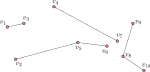
\includegraphics[width=0.75\textwidth]{segments}
    \caption{Line Segments for Trapezoidal Map}
\end{figure}

Note:
The vertices are labeled by increasing $x$-coordinate.  I also suggest that you
use the SVG file to help you with the illustrations of each step along the way.

\paragraph{Answer}

\todo{replace this TODO with your answer}

%%%%%%%%%%%%%%%%%%%%%%%%%%%%%%%%%%%%%%%%%%%%%%%%%%%%%%%%%%%%%%%%%%%%%%%%%%%%%%

%%%%%%%%%%%%%%%%%%%%%%%%%%%%%%%%%%%%%%%%%%%%%%%%%%%%%%%%%%%%%%%%%%%%%%%%%%%%%%
\collab{\todo{}}
\nextprob{Reflection}

Explain to me anything that you tried differently on this homework, focused on
for improvement of technical writing, or what you would especially like feedback
on.  It can be something simple like ``Before this class, I was not very aware
of what tense I was writing in.  For this homework, I tried to focus on writing
in present tense.'' or something very focused, such as ``I really focused on
improving my End-condition proofs for loop invariants.''  If you tried something
and struggled, let me know. Since everyone needs to improve (including me),
there should be something that you can write about here.  You can base it on
feedback I gave you, feedback I gave the class, feedback you received from
someone else, an example of technical writing that you really liked, or anything
else that motivates you to improve.

\paragraph{Answer}

\todo{replace this TODO with your answer}
%%%%%%%%%%%%%%%%%%%%%%%%%%%%%%%%%%%%%%%%%%%%%%%%%%%%%%%%%%%%%%%%%%%%%%%%%%%%%%

\end{document}
